% Options for packages loaded elsewhere
% Options for packages loaded elsewhere
\PassOptionsToPackage{unicode}{hyperref}
\PassOptionsToPackage{hyphens}{url}
\PassOptionsToPackage{dvipsnames,svgnames,x11names}{xcolor}
%
\documentclass[
  a4paper,
]{article}
\usepackage{xcolor}
\usepackage{amsmath,amssymb}
\setcounter{secnumdepth}{-\maxdimen} % remove section numbering
\usepackage{iftex}
\ifPDFTeX
  \usepackage[T1]{fontenc}
  \usepackage[utf8]{inputenc}
  \usepackage{textcomp} % provide euro and other symbols
\else % if luatex or xetex
  \usepackage{unicode-math} % this also loads fontspec
  \defaultfontfeatures{Scale=MatchLowercase}
  \defaultfontfeatures[\rmfamily]{Ligatures=TeX,Scale=1}
\fi
\usepackage{lmodern}
\ifPDFTeX\else
  % xetex/luatex font selection
\fi
% Use upquote if available, for straight quotes in verbatim environments
\IfFileExists{upquote.sty}{\usepackage{upquote}}{}
\IfFileExists{microtype.sty}{% use microtype if available
  \usepackage[]{microtype}
  \UseMicrotypeSet[protrusion]{basicmath} % disable protrusion for tt fonts
}{}
\makeatletter
\@ifundefined{KOMAClassName}{% if non-KOMA class
  \IfFileExists{parskip.sty}{%
    \usepackage{parskip}
  }{% else
    \setlength{\parindent}{0pt}
    \setlength{\parskip}{6pt plus 2pt minus 1pt}}
}{% if KOMA class
  \KOMAoptions{parskip=half}}
\makeatother
% Make \paragraph and \subparagraph free-standing
\makeatletter
\ifx\paragraph\undefined\else
  \let\oldparagraph\paragraph
  \renewcommand{\paragraph}{
    \@ifstar
      \xxxParagraphStar
      \xxxParagraphNoStar
  }
  \newcommand{\xxxParagraphStar}[1]{\oldparagraph*{#1}\mbox{}}
  \newcommand{\xxxParagraphNoStar}[1]{\oldparagraph{#1}\mbox{}}
\fi
\ifx\subparagraph\undefined\else
  \let\oldsubparagraph\subparagraph
  \renewcommand{\subparagraph}{
    \@ifstar
      \xxxSubParagraphStar
      \xxxSubParagraphNoStar
  }
  \newcommand{\xxxSubParagraphStar}[1]{\oldsubparagraph*{#1}\mbox{}}
  \newcommand{\xxxSubParagraphNoStar}[1]{\oldsubparagraph{#1}\mbox{}}
\fi
\makeatother


\usepackage{longtable,booktabs,array}
\usepackage{calc} % for calculating minipage widths
% Correct order of tables after \paragraph or \subparagraph
\usepackage{etoolbox}
\makeatletter
\patchcmd\longtable{\par}{\if@noskipsec\mbox{}\fi\par}{}{}
\makeatother
% Allow footnotes in longtable head/foot
\IfFileExists{footnotehyper.sty}{\usepackage{footnotehyper}}{\usepackage{footnote}}
\makesavenoteenv{longtable}
\usepackage{graphicx}
\makeatletter
\newsavebox\pandoc@box
\newcommand*\pandocbounded[1]{% scales image to fit in text height/width
  \sbox\pandoc@box{#1}%
  \Gscale@div\@tempa{\textheight}{\dimexpr\ht\pandoc@box+\dp\pandoc@box\relax}%
  \Gscale@div\@tempb{\linewidth}{\wd\pandoc@box}%
  \ifdim\@tempb\p@<\@tempa\p@\let\@tempa\@tempb\fi% select the smaller of both
  \ifdim\@tempa\p@<\p@\scalebox{\@tempa}{\usebox\pandoc@box}%
  \else\usebox{\pandoc@box}%
  \fi%
}
% Set default figure placement to htbp
\def\fps@figure{htbp}
\makeatother





\setlength{\emergencystretch}{3em} % prevent overfull lines

\providecommand{\tightlist}{%
  \setlength{\itemsep}{0pt}\setlength{\parskip}{0pt}}



 


\makeatletter
\@ifpackageloaded{caption}{}{\usepackage{caption}}
\AtBeginDocument{%
\ifdefined\contentsname
  \renewcommand*\contentsname{Table of contents}
\else
  \newcommand\contentsname{Table of contents}
\fi
\ifdefined\listfigurename
  \renewcommand*\listfigurename{List of Figures}
\else
  \newcommand\listfigurename{List of Figures}
\fi
\ifdefined\listtablename
  \renewcommand*\listtablename{List of Tables}
\else
  \newcommand\listtablename{List of Tables}
\fi
\ifdefined\figurename
  \renewcommand*\figurename{Figure}
\else
  \newcommand\figurename{Figure}
\fi
\ifdefined\tablename
  \renewcommand*\tablename{Table}
\else
  \newcommand\tablename{Table}
\fi
}
\@ifpackageloaded{float}{}{\usepackage{float}}
\floatstyle{ruled}
\@ifundefined{c@chapter}{\newfloat{codelisting}{h}{lop}}{\newfloat{codelisting}{h}{lop}[chapter]}
\floatname{codelisting}{Listing}
\newcommand*\listoflistings{\listof{codelisting}{List of Listings}}
\makeatother
\makeatletter
\makeatother
\makeatletter
\@ifpackageloaded{caption}{}{\usepackage{caption}}
\@ifpackageloaded{subcaption}{}{\usepackage{subcaption}}
\makeatother
\usepackage{bookmark}
\IfFileExists{xurl.sty}{\usepackage{xurl}}{} % add URL line breaks if available
\urlstyle{same}
\hypersetup{
  pdftitle={The Simpsons Viewership Analysis},
  colorlinks=true,
  linkcolor={blue},
  filecolor={Maroon},
  citecolor={Blue},
  urlcolor={Blue},
  pdfcreator={LaTeX via pandoc}}


\title{The Simpsons Viewership Analysis}
\author{}
\date{}
\begin{document}
\maketitle

\renewcommand*\contentsname{Table of contents}
{
\hypersetup{linkcolor=}
\setcounter{tocdepth}{3}
\tableofcontents
}

\subsection{1. Show Description}\label{show-description}

\emph{The Simpsons} is an American animated sitcom created by Matt
Groening that premiered on December 17, 1989. The series follows the
satirical adventures of the Simpson family - Homer, Marge, Bart, Lisa,
and Maggie - in the fictional town of Springfield. As the
longest-running American scripted primetime television series, it has
become a cultural phenomenon.

\subsection{2. Logo representation}\label{logo-representation}

\begin{verbatim}
<IPython.core.display.HTML object>
\end{verbatim}

\subsection{3. Basic Statistics}\label{basic-statistics}

\begin{longtable}[]{@{}ll@{}}

\caption{\label{tbl-stats}Basic Statistics}

\tabularnewline

\caption{}\label{T_27ee7}\tabularnewline
\toprule\noalign{}
Metric & Value \\
\midrule\noalign{}
\endfirsthead
\toprule\noalign{}
Metric & Value \\
\midrule\noalign{}
\endhead
\bottomrule\noalign{}
\endlastfoot
Seasons & 36 \\
Episodes & 782 \\
Peak Viewership & 33.6 million (S3E1, 1991) \\
Current Viewership & 1.2 million (S35) \\
IMDb Rating & 8.6/10 \\

\end{longtable}

\subsection{4. Viewership Trend}\label{viewership-trend}

\begin{figure}

\centering{

\pandocbounded{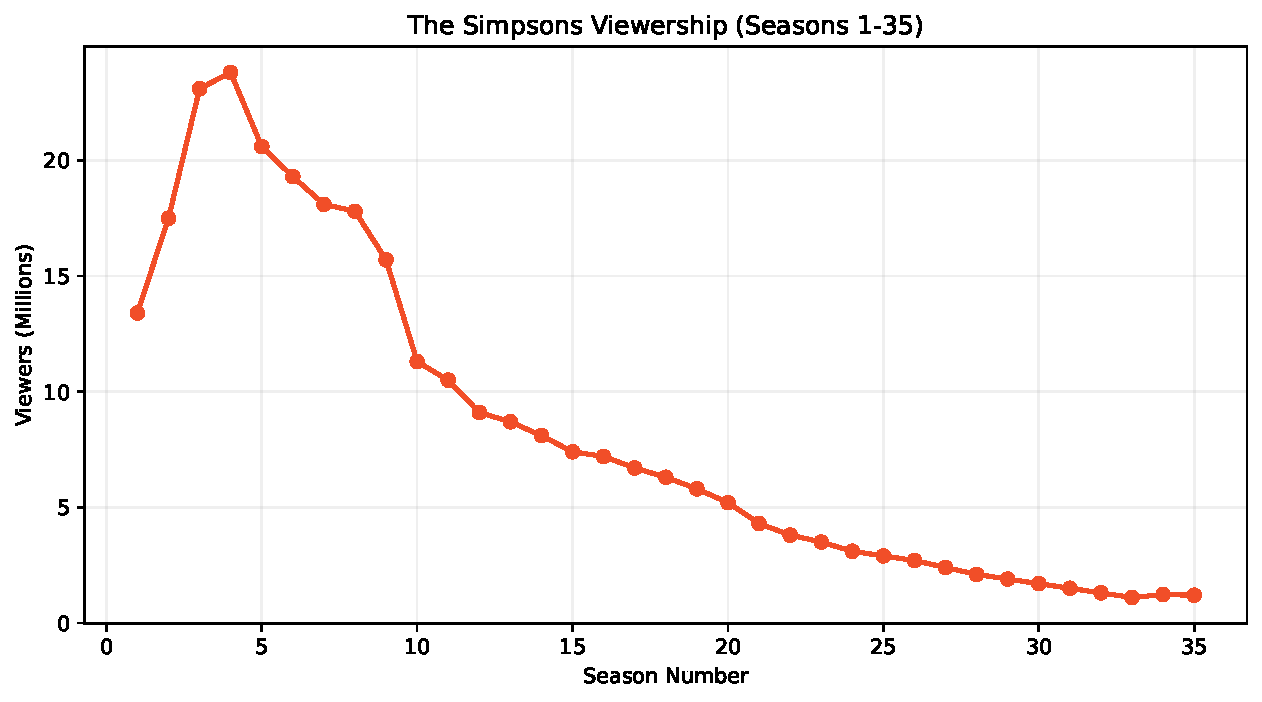
\includegraphics[keepaspectratio]{Simpsons_a7_files/figure-pdf/fig-trend-output-1.pdf}}

}

\caption{\label{fig-trend}Average Seasonal Viewership (Millions)}

\end{figure}%

\subsection{5. Yearly Changes}\label{yearly-changes}

\begin{figure}

\centering{

\pandocbounded{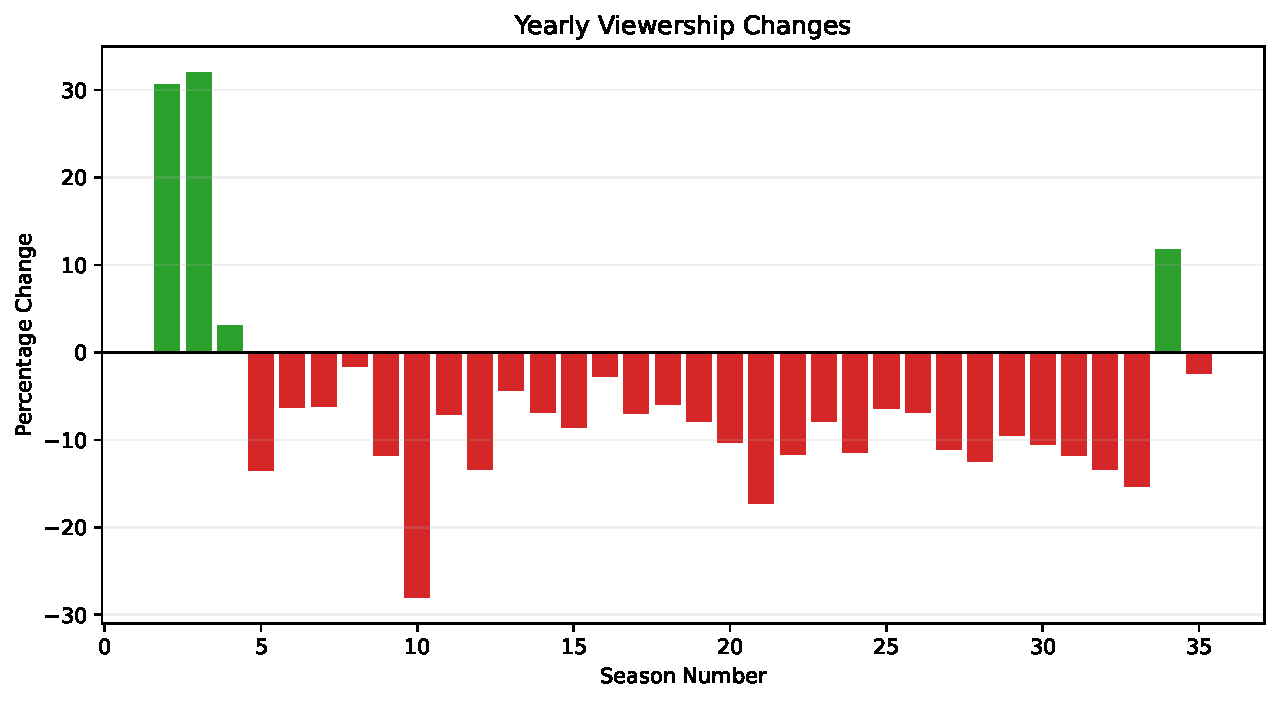
\includegraphics[keepaspectratio]{Simpsons_a7_files/figure-pdf/fig-changes-output-1.pdf}}

}

\caption{\label{fig-changes}Season-to-Season Viewership Changes (\%)}

\end{figure}%

\subsection{6. Trend Analysis}\label{trend-analysis}

The viewership data reveals several significant patterns in \emph{The
Simpsons'} audience trends over its 35-season run:

\textbf{Peak Performance Era}

The show reached its highest popularity during \textbf{Season 3}
(1991-92), averaging \textbf{23.1 million viewers} per episode. This
represented a dramatic \textbf{72.4\% increase} from Season 1's average,
demonstrating the series' rapid growth in its early years.

\textbf{Critical Decline Period}

The most substantial viewership drop occurred between \textbf{Seasons
9-10} (1997-99), with a \textbf{28.0\% decrease} in average viewership.
This coincided with: - Increased competition from other animated series
- Changes in writing staff - Shifting audience preferences

\textbf{Modern Era Stability}

In recent seasons (31-35), the show has stabilized with: - An average of
\textbf{1.3 million viewers} - Seasonal fluctuations of
\textbf{±15.4\%}\\
While significantly lower than peak numbers, this demonstrates the
series maintains a loyal core audience.

\textbf{Long-Term Trend}

The overall \textbf{91.0\% decline} from Season 1 to Season 35 reflects
both: 1. Natural aging of a long-running series 2. Fundamental changes
in television viewing habits 3. Increased competition in the streaming
era

\emph{Despite these declines, The Simpsons remains culturally
significant and profitable through syndication and streaming deals.}

\subsection{References}\label{references}

\subsubsection{Data Sources}\label{data-sources}

\begin{enumerate}
\def\labelenumi{\arabic{enumi}.}
\tightlist
\item
  \href{https://en.wikipedia.org/wiki/List_of_The_Simpsons_episodes}{The
  Simpsons Episode Guide}, Wikipedia\\
\item
  \href{https://www.imdb.com/title/tt0096697/episodes}{IMDb Episode
  Ratings}, IMDb
\end{enumerate}

\subsubsection{Image Credits}\label{image-credits}

\begin{itemize}
\tightlist
\item
  Logo:
  \href{https://upload.wikimedia.org/wikipedia/commons/thumb/b/b7/The_logo_simpsons_yellow.png/1200px-The_logo_simpsons_yellow.png?20210413044310}{Fair
  use via Wikimedia}
\end{itemize}




\end{document}
